
% This LaTeX was auto-generated from MATLAB code.
% To make changes, update the MATLAB code and republish this document.

\documentclass{article}
\usepackage{graphicx}
\usepackage{color}

\sloppy
\definecolor{lightgray}{gray}{0.5}
\setlength{\parindent}{0pt}

\begin{document}

    
    
\section*{MATLAB programming course for beginners, supported by Wagatsuma Lab@Kyutech}

\begin{par}
/* The MIT License (MIT): Copyright (c) 2017 Hiroaki Wagatsuma and Wagatsuma Lab@Kyutech
\end{par} \vspace{1em}
\begin{par}
Permission is hereby granted, free of charge, to any person obtaining a copy of this software and associated documentation files (the "Software"), to deal in the Software without restriction, including without limitation the rights to use, copy, modify, merge, publish, distribute, sublicense, and/or sell copies of the Software, and to permit persons to whom the Software is furnished to do so, subject to the following conditions:
\end{par} \vspace{1em}
\begin{par}
The above copyright notice and this permission notice shall be included in all copies or substantial portions of the Software.
\end{par} \vspace{1em}
\begin{par}
THE SOFTWARE IS PROVIDED "AS IS", WITHOUT WARRANTY OF ANY KIND, EXPRESS OR IMPLIED, INCLUDING BUT NOT LIMITED TO THE WARRANTIES OF MERCHANTABILITY, FITNESS FOR A PARTICULAR PURPOSE AND NONINFRINGEMENT. IN NO EVENT SHALL THE AUTHORS OR COPYRIGHT HOLDERS BE LIABLE FOR ANY CLAIM, DAMAGES OR OTHER LIABILITY, WHETHER IN AN ACTION OF CONTRACT, TORT OR OTHERWISE, ARISING FROM, OUT OF OR IN CONNECTION WITH THE SOFTWARE OR THE USE OR OTHER DEALINGS IN THE SOFTWARE. */
\end{par} \vspace{1em}

\subsection*{Contents}

\begin{itemize}
\setlength{\itemsep}{-1ex}
   \item Specifications and requirements
   \item Main program
\end{itemize}


\subsection*{Specifications and requirements}

\begin{enumerate}
\setlength{\itemsep}{-1ex}
   \item @Time    : 2017-2-20
   \item @Author  : Hiroaki Wagatsuma
   \item @Site    : https://github.com/hirowgit/1B1\_matlab\_signal\_analysis\_course
   \item @IDE     : MATLAB R2018a
   \item @File    : readEEG\_Gold.m
\end{enumerate}


\subsection*{Main program}

\begin{par}
clear all
\end{par} \vspace{1em}
\begin{verbatim}
clc
% clear all;
currdir=pwd;

Tnum=1;
source_F={'A-Z','B-O','C-N','D-F','E-S'};
output_F={'outA-Z','outB-O','outC-N','outD-F','outE-S'};
source_Lname={'awake state when eyes were opening','awake state when eyes were closed','Presurgical + opposite zone','Presurgical + epileptogenic zone','contained seizure activity'};
source_L2name={'eye-opening','eye-closed','opposite presurgical','epileptogenic presurgical','seizure activity'};

DataFolder='';
if ~isdir(source_F{1})
    prompt = 'Please specify the path of the data folders such as "A-Z","B-O","C-N","D-F","E-S": ';
    DataFolder = input(prompt,'s');
end

all_fft=[];
for Tnum=1:length(source_F)

source_folder=fullfile(DataFolder,source_F{Tnum}); close all
output_folder=output_F{Tnum};
% source_file='Z001raw.txt';
% fname=fullfile(source_folder,source_file);
% output_folder='eeg_analyzed';
if ~exist('fignum','var'); fignum=0; end

fignum=0;
close all;
readingAllmarge_Copper;

%All EEG signals were recorded with the same 128- channel amplifier system,
% using an average common refer- ence ?omitting electrodes containing pathological activity ?C, D, and E
% ? or strong eye movement artifacts ?A and B??. After 12 bit analog-to-digital conversion, the data were written continuou
% sly onto the disk of a data acquisition computer system at a sampling rate of 173.61 Hz. Band-pass filter settings were 0.53 ? 40 Hz ?12 dB/oct.?.

%
% cd(source_folder);

ntag={'time','original','filtered'};
% eegdata=importdata(fname);
eegdata=data_all;

% tstamp=eegdata(:,1);
tstamp=importdata('timeline.txt');

fignum=fignum+1;figure(fignum);  clf
plot(tstamp,eegdata(:,2),tstamp,eegdata(:,3));

fnn=['ts_',source_folder]; fnn=strrep(fnn, '-', '_');
set(fignum,'name',fnn);


    N           = length(tstamp);
    n           = 2^(nextpow2(N-1));
    eegsignal = eegdata(1:N,:);

%
%     [mx,nx] = size(eegsignal);
%
%   d = max(mx,nx);

fs=173.61;
T=1/fs;
% yrange=[0 200];
yrange=[0 50];
yrange=[50 150];

xrange=[0 50];
xrange=[0 80];

eegs_fft=eegsignal;
fftdata=fft(eegs_fft,fs);
Cut_fft=[fftdata(1: floor(fs/2)+1,:)];
% Cut_fft=fftdata;
mag_abs=abs(Cut_fft);

freq=([0:fs/2]./(fs*T))';
freqs=repmat(freq,[1,3]);
axis_name={'Frequency (Hz)','Amplitude'};

fignum=fignum+1;figure(fignum);  clf
% ttext={'Separation of frequency '};
%s=['*','x','0','+','s','D'];
hold on
%for k2=1:6

%     plot(freq,20*log10(mag_abs(:,1)),'--go',freq,20*log10(mag_abs(:,2)),': r * ');
%     plot(20*log10(mag_abs(:,1:3)));
    plot(freq,20*log10(mag_abs));
    title(source_Lname{Tnum});

    fnn=['fft_',source_folder]; fnn=strrep(fnn, '-', '_');
    set(fignum,'name',fnn);
    xlabel('Frequency(Hz)');
    ylabel('Power');
%   set(gca,'XLabel',axis_name{1});
 %   set(gca,'YLabel',axis_name{2});
%     set(gca,'ylim',yrange,'xlim',xrange);
        set(gca,'xlim',xrange);
grid on;


    fignum=fignum+1;figure(fignum);  clf
    mag_ave=(sum(mag_abs')./size(data_all,2))';

    plot(freq,20*log10(mag_ave));
    title(source_Lname{Tnum});

    fnn=['fft_average_',source_folder]; fnn=strrep(fnn, '-', '_');
    set(fignum,'name',fnn);
    xlabel('Frequency(Hz)');
    ylabel('Power');
%     set(gca,'ylim',yrange,'xlim',xrange);
    set(gca,'xlim',xrange);
    grid on;

    all_fft(:,Tnum)=mag_ave;
%   Hleg1 = legend (  'gamma','beta','alpha','theta','delta','EOG' );
%   Hleg1 = legend (  'original','filtered' );
% hold off

datafname=output_folder;
save_fig;
cd(output_folder);
save(fout2_name,'data_all','-ascii','-tabs');
cd(currdir);

end

close all;
    fignum=fignum+1;figure(fignum);  clf
    mag_ave=(sum(mag_abs')./size(data_all,2))';

    plot(freq,20*log10(all_fft));
    title('FFT Comparison');

    fnn=['fft_all_',source_folder]; fnn=strrep(fnn, '-', '_');
    set(fignum,'name',fnn);
    xlabel('Frequency(Hz)');
    ylabel('Power');
%     set(gca,'ylim',yrange,'xlim',xrange);
        set(gca,'xlim',xrange);
grid on;

%     all_fft(:,Tnum)=mag_ave;

    Hleg1 = legend (source_L2name);
    datafname='out_all';
save_fig;
\end{verbatim}

        \color{lightgray} \begin{verbatim}
flist =

  1�~100 cell array

  Columns 1 through 4

    {'Z001.txt'}    {'Z002.txt'}    {'Z003.txt'}    {'Z004.txt'}

  Columns 5 through 8

    {'Z005.txt'}    {'Z006.txt'}    {'Z007.txt'}    {'Z008.txt'}

  Columns 9 through 12

    {'Z009.txt'}    {'Z010.txt'}    {'Z011.txt'}    {'Z012.txt'}

  Columns 13 through 16

    {'Z013.txt'}    {'Z014.txt'}    {'Z015.txt'}    {'Z016.txt'}

  Columns 17 through 20

    {'Z017.txt'}    {'Z018.txt'}    {'Z019.txt'}    {'Z020.txt'}

  Columns 21 through 24

    {'Z021.txt'}    {'Z022.txt'}    {'Z023.txt'}    {'Z024.txt'}

  Columns 25 through 28

    {'Z025.txt'}    {'Z026.txt'}    {'Z027.txt'}    {'Z028.txt'}

  Columns 29 through 32

    {'Z029.txt'}    {'Z030.txt'}    {'Z031.txt'}    {'Z032.txt'}

  Columns 33 through 36

    {'Z033.txt'}    {'Z034.txt'}    {'Z035.txt'}    {'Z036.txt'}

  Columns 37 through 40

    {'Z037.txt'}    {'Z038.txt'}    {'Z039.txt'}    {'Z040.txt'}

  Columns 41 through 44

    {'Z041.txt'}    {'Z042.txt'}    {'Z043.txt'}    {'Z044.txt'}

  Columns 45 through 48

    {'Z045.txt'}    {'Z046.txt'}    {'Z047.txt'}    {'Z048.txt'}

  Columns 49 through 52

    {'Z049.txt'}    {'Z050.txt'}    {'Z051.txt'}    {'Z052.txt'}

  Columns 53 through 56

    {'Z053.txt'}    {'Z054.txt'}    {'Z055.txt'}    {'Z056.txt'}

  Columns 57 through 60

    {'Z057.txt'}    {'Z058.txt'}    {'Z059.txt'}    {'Z060.txt'}

  Columns 61 through 64

    {'Z061.txt'}    {'Z062.txt'}    {'Z063.txt'}    {'Z064.txt'}

  Columns 65 through 68

    {'Z065.txt'}    {'Z066.txt'}    {'Z067.txt'}    {'Z068.txt'}

  Columns 69 through 72

    {'Z069.txt'}    {'Z070.txt'}    {'Z071.txt'}    {'Z072.txt'}

  Columns 73 through 76

    {'Z073.txt'}    {'Z074.txt'}    {'Z075.txt'}    {'Z076.txt'}

  Columns 77 through 80

    {'Z077.txt'}    {'Z078.txt'}    {'Z079.txt'}    {'Z080.txt'}

  Columns 81 through 84

    {'Z081.txt'}    {'Z082.txt'}    {'Z083.txt'}    {'Z084.txt'}

  Columns 85 through 88

    {'Z085.txt'}    {'Z086.txt'}    {'Z087.txt'}    {'Z088.txt'}

  Columns 89 through 92

    {'Z089.txt'}    {'Z090.txt'}    {'Z091.txt'}    {'Z092.txt'}

  Columns 93 through 96

    {'Z093.txt'}    {'Z094.txt'}    {'Z095.txt'}    {'Z096.txt'}

  Columns 97 through 100

    {'Z097.txt'}    {'Z098.txt'}    {'Z099.txt'}    {'Z100.txt'}

        4097         100

Warning: FFT length must be a nonnegative integer scalar. 

flist =

  1�~100 cell array

  Columns 1 through 4

    {'O001.txt'}    {'O002.txt'}    {'O003.txt'}    {'O004.txt'}

  Columns 5 through 8

    {'O005.txt'}    {'O006.txt'}    {'O007.txt'}    {'O008.txt'}

  Columns 9 through 12

    {'O009.txt'}    {'O010.txt'}    {'O011.txt'}    {'O012.txt'}

  Columns 13 through 16

    {'O013.txt'}    {'O014.txt'}    {'O015.txt'}    {'O016.txt'}

  Columns 17 through 20

    {'O017.txt'}    {'O018.txt'}    {'O019.txt'}    {'O020.txt'}

  Columns 21 through 24

    {'O021.txt'}    {'O022.txt'}    {'O023.txt'}    {'O024.txt'}

  Columns 25 through 28

    {'O025.txt'}    {'O026.txt'}    {'O027.txt'}    {'O028.txt'}

  Columns 29 through 32

    {'O029.txt'}    {'O030.txt'}    {'O031.txt'}    {'O032.txt'}

  Columns 33 through 36

    {'O033.txt'}    {'O034.txt'}    {'O035.txt'}    {'O036.txt'}

  Columns 37 through 40

    {'O037.txt'}    {'O038.txt'}    {'O039.txt'}    {'O040.txt'}

  Columns 41 through 44

    {'O041.txt'}    {'O042.txt'}    {'O043.txt'}    {'O044.txt'}

  Columns 45 through 48

    {'O045.txt'}    {'O046.txt'}    {'O047.txt'}    {'O048.txt'}

  Columns 49 through 52

    {'O049.txt'}    {'O050.txt'}    {'O051.txt'}    {'O052.txt'}

  Columns 53 through 56

    {'O053.txt'}    {'O054.txt'}    {'O055.txt'}    {'O056.txt'}

  Columns 57 through 60

    {'O057.txt'}    {'O058.txt'}    {'O059.txt'}    {'O060.txt'}

  Columns 61 through 64

    {'O061.txt'}    {'O062.txt'}    {'O063.txt'}    {'O064.txt'}

  Columns 65 through 68

    {'O065.txt'}    {'O066.txt'}    {'O067.txt'}    {'O068.txt'}

  Columns 69 through 72

    {'O069.txt'}    {'O070.txt'}    {'O071.txt'}    {'O072.txt'}

  Columns 73 through 76

    {'O073.txt'}    {'O074.txt'}    {'O075.txt'}    {'O076.txt'}

  Columns 77 through 80

    {'O077.txt'}    {'O078.txt'}    {'O079.txt'}    {'O080.txt'}

  Columns 81 through 84

    {'O081.txt'}    {'O082.txt'}    {'O083.txt'}    {'O084.txt'}

  Columns 85 through 88

    {'O085.txt'}    {'O086.txt'}    {'O087.txt'}    {'O088.txt'}

  Columns 89 through 92

    {'O089.txt'}    {'O090.txt'}    {'O091.txt'}    {'O092.txt'}

  Columns 93 through 96

    {'O093.txt'}    {'O094.txt'}    {'O095.txt'}    {'O096.txt'}

  Columns 97 through 100

    {'O097.txt'}    {'O098.txt'}    {'O099.txt'}    {'O100.txt'}

        4097         100

Warning: FFT length must be a nonnegative integer scalar. 

flist =

  1�~100 cell array

  Columns 1 through 4

    {'N001.TXT'}    {'N002.TXT'}    {'N003.TXT'}    {'N004.TXT'}

  Columns 5 through 8

    {'N005.TXT'}    {'N006.TXT'}    {'N007.TXT'}    {'N008.TXT'}

  Columns 9 through 12

    {'N009.TXT'}    {'N010.TXT'}    {'N011.TXT'}    {'N012.TXT'}

  Columns 13 through 16

    {'N013.TXT'}    {'N014.TXT'}    {'N015.TXT'}    {'N016.TXT'}

  Columns 17 through 20

    {'N017.TXT'}    {'N018.TXT'}    {'N019.TXT'}    {'N020.TXT'}

  Columns 21 through 24

    {'N021.TXT'}    {'N022.TXT'}    {'N023.TXT'}    {'N024.TXT'}

  Columns 25 through 28

    {'N025.TXT'}    {'N026.TXT'}    {'N027.TXT'}    {'N028.TXT'}

  Columns 29 through 32

    {'N029.TXT'}    {'N030.TXT'}    {'N031.TXT'}    {'N032.TXT'}

  Columns 33 through 36

    {'N033.TXT'}    {'N034.TXT'}    {'N035.TXT'}    {'N036.TXT'}

  Columns 37 through 40

    {'N037.TXT'}    {'N038.TXT'}    {'N039.TXT'}    {'N040.TXT'}

  Columns 41 through 44

    {'N041.TXT'}    {'N042.TXT'}    {'N043.TXT'}    {'N044.TXT'}

  Columns 45 through 48

    {'N045.TXT'}    {'N046.TXT'}    {'N047.TXT'}    {'N048.TXT'}

  Columns 49 through 52

    {'N049.TXT'}    {'N050.TXT'}    {'N051.TXT'}    {'N052.TXT'}

  Columns 53 through 56

    {'N053.TXT'}    {'N054.TXT'}    {'N055.TXT'}    {'N056.TXT'}

  Columns 57 through 60

    {'N057.TXT'}    {'N058.TXT'}    {'N059.TXT'}    {'N060.TXT'}

  Columns 61 through 64

    {'N061.TXT'}    {'N062.TXT'}    {'N063.TXT'}    {'N064.TXT'}

  Columns 65 through 68

    {'N065.TXT'}    {'N066.TXT'}    {'N067.TXT'}    {'N068.TXT'}

  Columns 69 through 72

    {'N069.TXT'}    {'N070.TXT'}    {'N071.TXT'}    {'N072.TXT'}

  Columns 73 through 76

    {'N073.TXT'}    {'N074.TXT'}    {'N075.TXT'}    {'N076.TXT'}

  Columns 77 through 80

    {'N077.TXT'}    {'N078.TXT'}    {'N079.TXT'}    {'N080.TXT'}

  Columns 81 through 84

    {'N081.TXT'}    {'N082.TXT'}    {'N083.TXT'}    {'N084.TXT'}

  Columns 85 through 88

    {'N085.TXT'}    {'N086.TXT'}    {'N087.TXT'}    {'N088.TXT'}

  Columns 89 through 92

    {'N089.TXT'}    {'N090.TXT'}    {'N091.TXT'}    {'N092.TXT'}

  Columns 93 through 96

    {'N093.TXT'}    {'N094.TXT'}    {'N095.TXT'}    {'N096.TXT'}

  Columns 97 through 100

    {'N097.TXT'}    {'N098.TXT'}    {'N099.TXT'}    {'N100.TXT'}

        4097         100

Warning: FFT length must be a nonnegative integer scalar. 

flist =

  1�~100 cell array

  Columns 1 through 4

    {'F001.txt'}    {'F002.txt'}    {'F003.txt'}    {'F004.txt'}

  Columns 5 through 8

    {'F005.txt'}    {'F006.txt'}    {'F007.txt'}    {'F008.txt'}

  Columns 9 through 12

    {'F009.txt'}    {'F010.txt'}    {'F011.txt'}    {'F012.txt'}

  Columns 13 through 16

    {'F013.txt'}    {'F014.txt'}    {'F015.txt'}    {'F016.txt'}

  Columns 17 through 20

    {'F017.txt'}    {'F018.txt'}    {'F019.txt'}    {'F020.txt'}

  Columns 21 through 24

    {'F021.txt'}    {'F022.txt'}    {'F023.txt'}    {'F024.txt'}

  Columns 25 through 28

    {'F025.txt'}    {'F026.txt'}    {'F027.txt'}    {'F028.txt'}

  Columns 29 through 32

    {'F029.txt'}    {'F030.txt'}    {'F031.txt'}    {'F032.txt'}

  Columns 33 through 36

    {'F033.txt'}    {'F034.txt'}    {'F035.txt'}    {'F036.txt'}

  Columns 37 through 40

    {'F037.txt'}    {'F038.txt'}    {'F039.txt'}    {'F040.txt'}

  Columns 41 through 44

    {'F041.txt'}    {'F042.txt'}    {'F043.txt'}    {'F044.txt'}

  Columns 45 through 48

    {'F045.txt'}    {'F046.txt'}    {'F047.txt'}    {'F048.txt'}

  Columns 49 through 52

    {'F049.txt'}    {'F050.txt'}    {'F051.txt'}    {'F052.txt'}

  Columns 53 through 56

    {'F053.txt'}    {'F054.txt'}    {'F055.txt'}    {'F056.txt'}

  Columns 57 through 60

    {'F057.txt'}    {'F058.txt'}    {'F059.txt'}    {'F060.txt'}

  Columns 61 through 64

    {'F061.txt'}    {'F062.txt'}    {'F063.txt'}    {'F064.txt'}

  Columns 65 through 68

    {'F065.txt'}    {'F066.txt'}    {'F067.txt'}    {'F068.txt'}

  Columns 69 through 72

    {'F069.txt'}    {'F070.txt'}    {'F071.txt'}    {'F072.txt'}

  Columns 73 through 76

    {'F073.txt'}    {'F074.txt'}    {'F075.txt'}    {'F076.txt'}

  Columns 77 through 80

    {'F077.txt'}    {'F078.txt'}    {'F079.txt'}    {'F080.txt'}

  Columns 81 through 84

    {'F081.txt'}    {'F082.txt'}    {'F083.txt'}    {'F084.txt'}

  Columns 85 through 88

    {'F085.txt'}    {'F086.txt'}    {'F087.txt'}    {'F088.txt'}

  Columns 89 through 92

    {'F089.txt'}    {'F090.txt'}    {'F091.txt'}    {'F092.txt'}

  Columns 93 through 96

    {'F093.txt'}    {'F094.txt'}    {'F095.txt'}    {'F096.txt'}

  Columns 97 through 100

    {'F097.txt'}    {'F098.txt'}    {'F099.txt'}    {'F100.txt'}

        4097         100

Warning: FFT length must be a nonnegative integer scalar. 

flist =

  1�~100 cell array

  Columns 1 through 4

    {'S001.txt'}    {'S002.txt'}    {'S003.txt'}    {'S004.txt'}

  Columns 5 through 8

    {'S005.txt'}    {'S006.txt'}    {'S007.txt'}    {'S008.txt'}

  Columns 9 through 12

    {'S009.txt'}    {'S010.txt'}    {'S011.txt'}    {'S012.txt'}

  Columns 13 through 16

    {'S013.txt'}    {'S014.txt'}    {'S015.txt'}    {'S016.txt'}

  Columns 17 through 20

    {'S017.txt'}    {'S018.txt'}    {'S019.txt'}    {'S020.txt'}

  Columns 21 through 24

    {'S021.txt'}    {'S022.txt'}    {'S023.txt'}    {'S024.txt'}

  Columns 25 through 28

    {'S025.txt'}    {'S026.txt'}    {'S027.txt'}    {'S028.txt'}

  Columns 29 through 32

    {'S029.txt'}    {'S030.txt'}    {'S031.txt'}    {'S032.txt'}

  Columns 33 through 36

    {'S033.txt'}    {'S034.txt'}    {'S035.txt'}    {'S036.txt'}

  Columns 37 through 40

    {'S037.txt'}    {'S038.txt'}    {'S039.txt'}    {'S040.txt'}

  Columns 41 through 44

    {'S041.txt'}    {'S042.txt'}    {'S043.txt'}    {'S044.txt'}

  Columns 45 through 48

    {'S045.txt'}    {'S046.txt'}    {'S047.txt'}    {'S048.txt'}

  Columns 49 through 52

    {'S049.txt'}    {'S050.txt'}    {'S051.txt'}    {'S052.txt'}

  Columns 53 through 56

    {'S053.txt'}    {'S054.txt'}    {'S055.txt'}    {'S056.txt'}

  Columns 57 through 60

    {'S057.txt'}    {'S058.txt'}    {'S059.txt'}    {'S060.txt'}

  Columns 61 through 64

    {'S061.txt'}    {'S062.txt'}    {'S063.txt'}    {'S064.txt'}

  Columns 65 through 68

    {'S065.txt'}    {'S066.txt'}    {'S067.txt'}    {'S068.txt'}

  Columns 69 through 72

    {'S069.txt'}    {'S070.txt'}    {'S071.txt'}    {'S072.txt'}

  Columns 73 through 76

    {'S073.txt'}    {'S074.txt'}    {'S075.txt'}    {'S076.txt'}

  Columns 77 through 80

    {'S077.txt'}    {'S078.txt'}    {'S079.txt'}    {'S080.txt'}

  Columns 81 through 84

    {'S081.txt'}    {'S082.txt'}    {'S083.txt'}    {'S084.txt'}

  Columns 85 through 88

    {'S085.txt'}    {'S086.txt'}    {'S087.txt'}    {'S088.txt'}

  Columns 89 through 92

    {'S089.txt'}    {'S090.txt'}    {'S091.txt'}    {'S092.txt'}

  Columns 93 through 96

    {'S093.txt'}    {'S094.txt'}    {'S095.txt'}    {'S096.txt'}

  Columns 97 through 100

    {'S097.txt'}    {'S098.txt'}    {'S099.txt'}    {'S100.txt'}

        4097         100

Warning: FFT length must be a nonnegative integer scalar. 
\end{verbatim} \color{black}
    
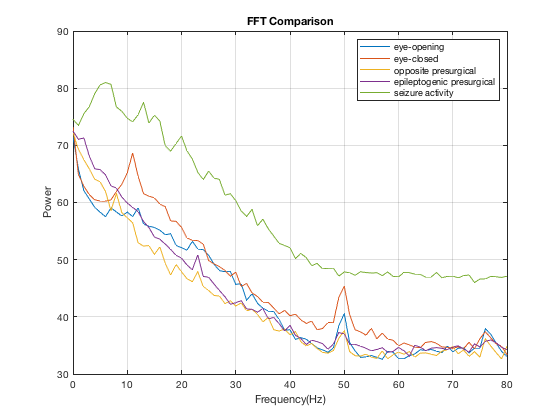
\includegraphics [width=4in]{freqPlotEEG_Gold_01.eps}



\end{document}
    
